\section{IO Tests}
Before our PCB board arrived we tested each subsystem separately.
During testing the group gained valuable experience about all the subcomponents and how they interacted with each others.

\subsection{DAC}

\subsubsection{Without the PCB}

The DAC was tested prior to PCB arrival, to ensure correct operation from an FPGA.
Eight wires were soldered onto the DAC, and connected to a breadboard.
The FPGA was flashed with and simple architecture, which repeatedly read the status of 14? general I/O pins, and shifted each bit out sequentially on another pin.
Both the DAC and FPGA clock input was driven by an external frequency generator, producing 3.3VPP at 10MHz.

To validate the signal output from the FPGA a logical analyser was used.

With VRef and VDD at 5.0V, the analogue DAC output was measured to 0.69V when no data signal was asserted, and 2.8V when the MSB was asserted. This small offset, is the result of some of the lower order bits being left unconnected.

\subsubsection{With the PCB}

Once the the PCB arrived we were able to test the DACs soldered onto the PCB as well as with actual data from the FPGA.

Clocking data from the FPGA to the DACs on our PCB presented some issues as we hit a limit in the Spartan 6 architecture regarding clock routing. This was resolved by using an ODDR\cite[pp. 61--65]{fpga-io} in order to forward the clock signal to the desired output pin.

Once we had the data input to the DACs working we could test the outputs. In does this we found some issues with out ground planes as well as the maximum output voltages from the DACs. The maximum voltage we were able to get was 1.6V, a little under half of our reference voltage of 3.3V. //TODO: Update this when the problem is fixed.


\subsection{Oscilloscope}
As a proof of concept to draw on an oscilloscope, we created a 4-bit resistor ladder DAC. The schematic of the DAC is displayed in Figure \ref{fig:r2r-ladder}.
An Arduino was used to control the DAC.

To test drawing on both x-axis and y-axis, the circuit consisted of 2 4-bit DACs.
With a small Arduino program we were able to draw a square, depicted in Figure \ref{fig:osc_poc}.
When the Arduino changed the voltage on its GPIO pins, there was a voltage drop across all pins.
The consequence of the voltage drop is clearly visible (see Figure \ref{fig:osc_poc}).


\begin{figure}[h]
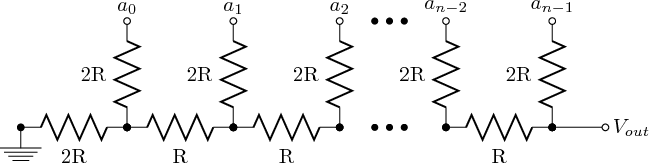
\includegraphics[width=\columnwidth]{images/r2r-ladder}
\centering
\caption{Schematics of the resistor-ladder\cite{r2r-ladder-schematics}.}
\label{fig:r2r-ladder}
\end{figure}

\begin{figure}[h]
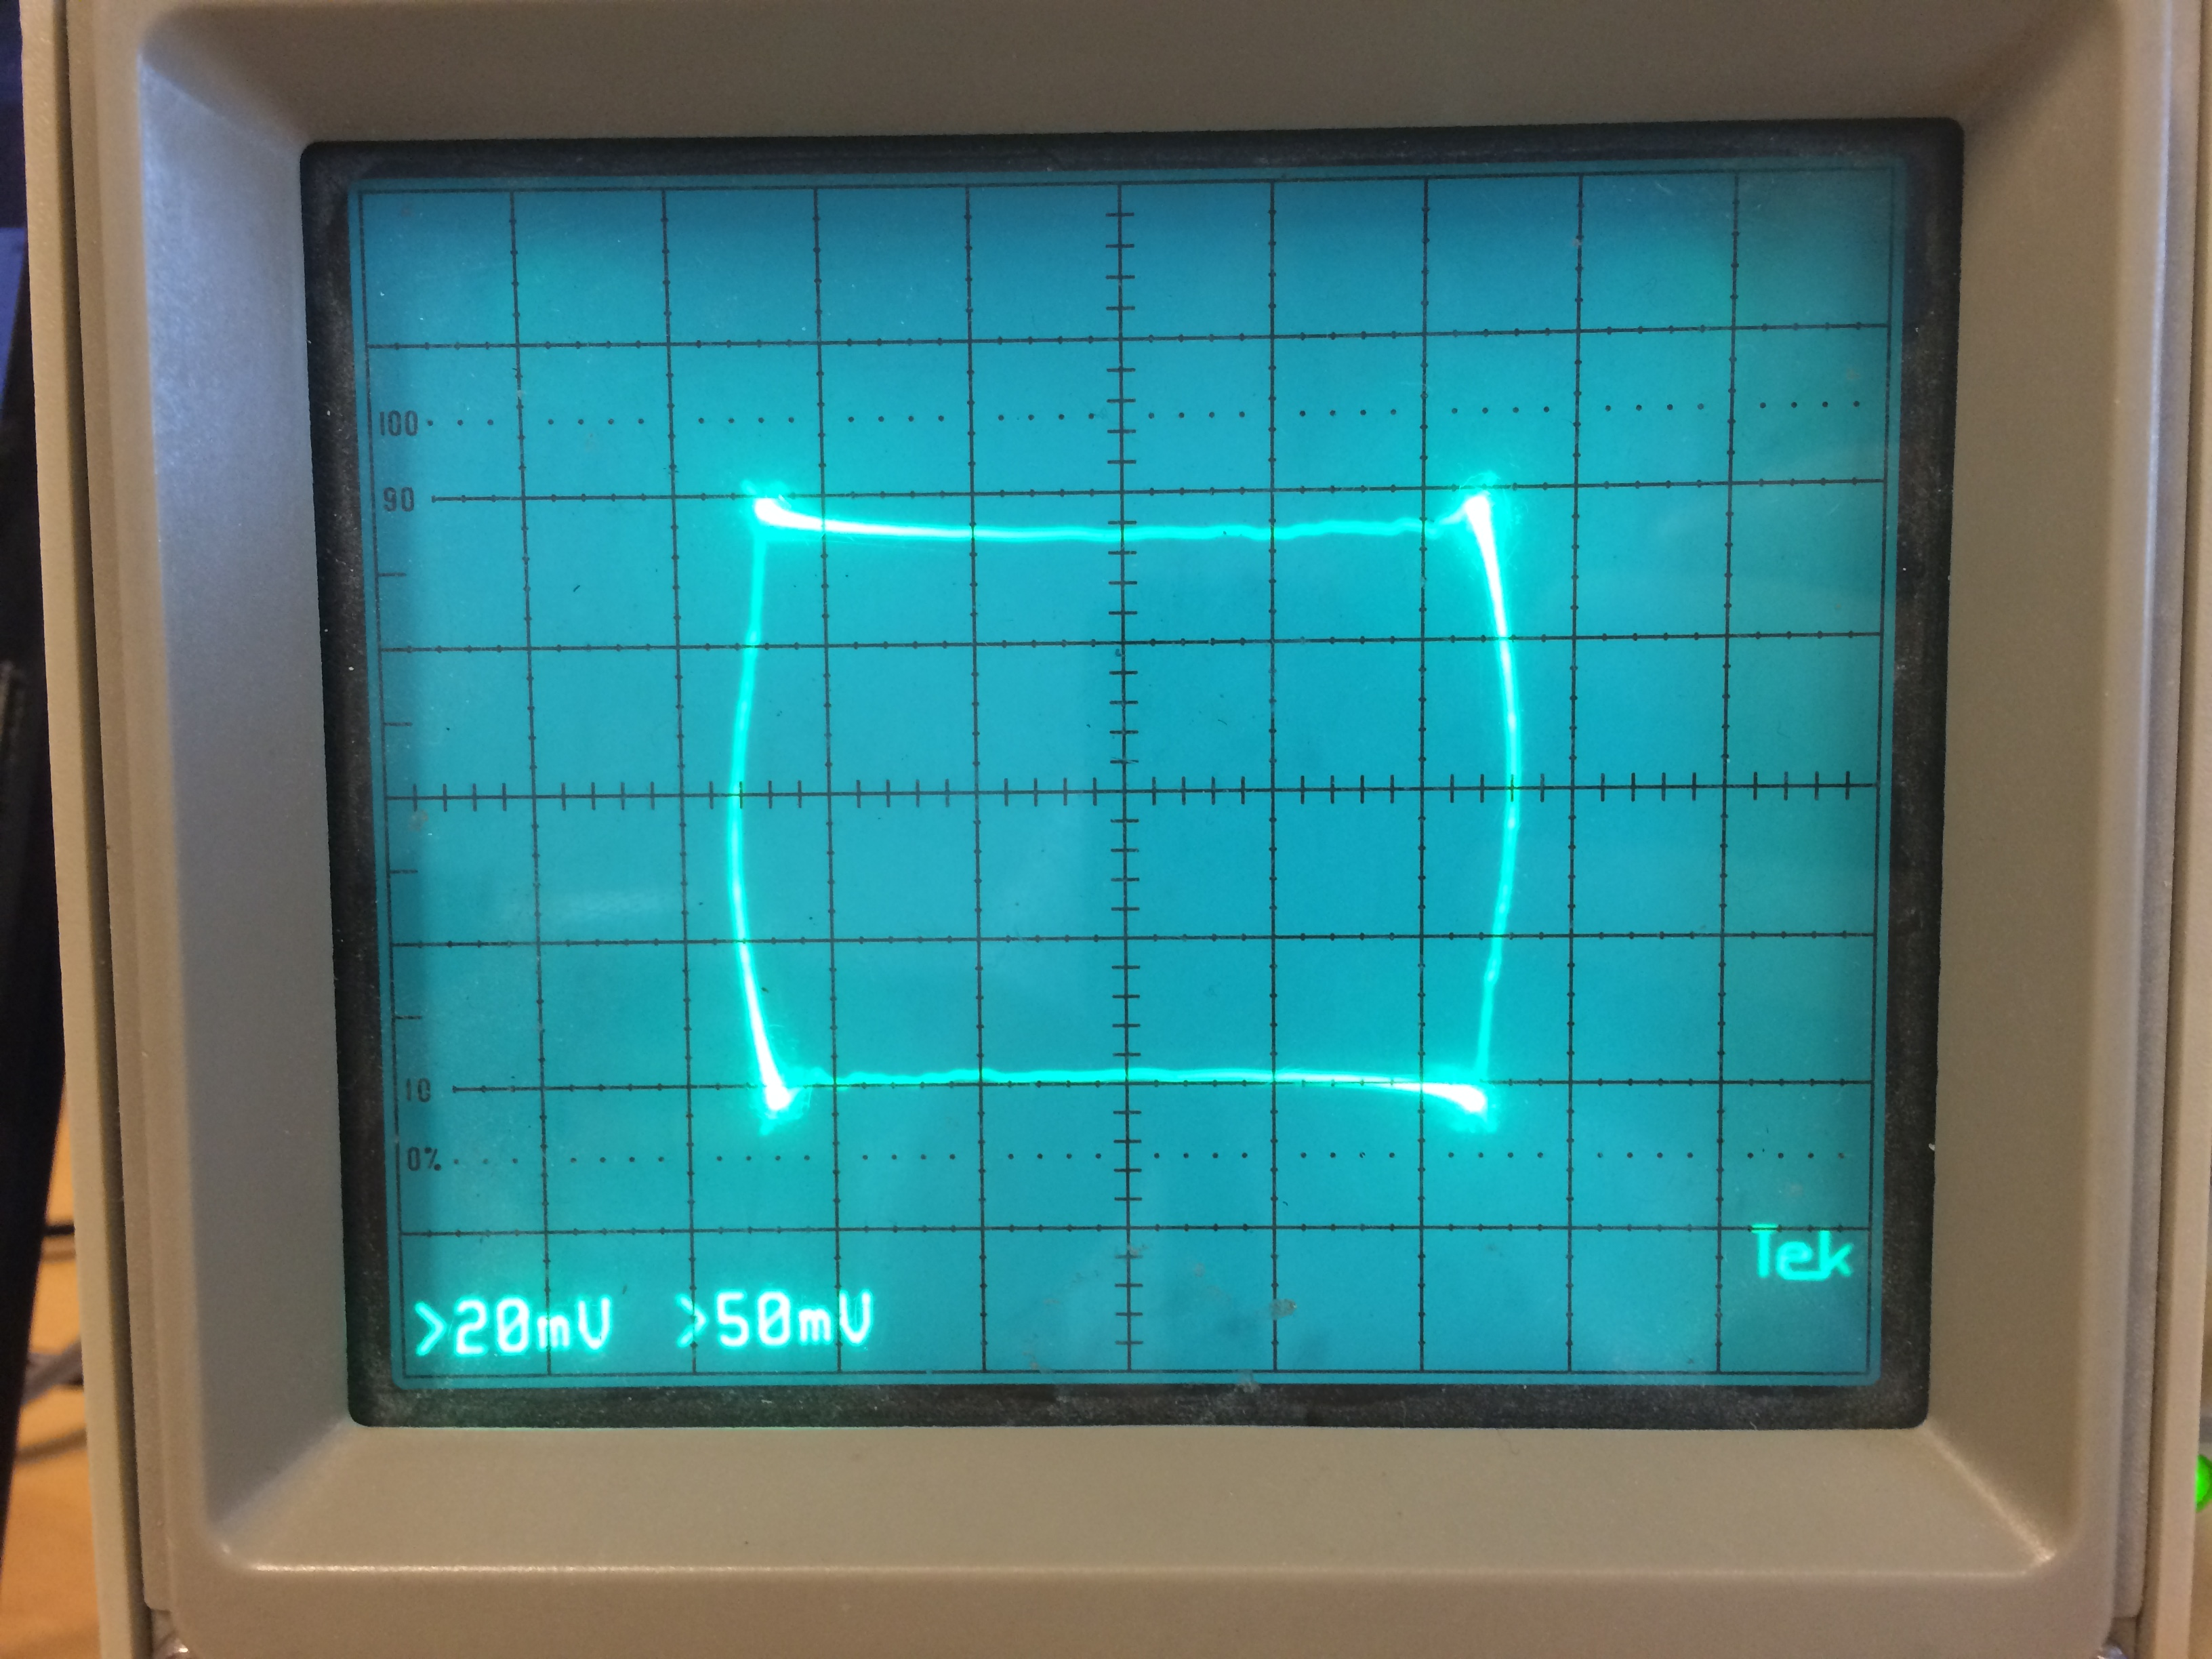
\includegraphics[width=\columnwidth]{images/osc_square_close}
\centering
\caption{A "square" drawn on the oscilloscope using an Arduino and two resistor-ladder DACs}
\label{fig:osc_poc}
\end{figure}